\chapter{Meshing}
\label{ref:mesh}

\section{What is meshing?}
Meshing is the process of taking a continuous problem space, say a bar along which heat is conducted form a candle to a block of ice and turning this into a discrete computational problem.  This usually involves picking a series of points along this space and using these to represent the entire problem (see Figure \ref{fig:emeshdiagram}). The reason we need to break a region up into points to model it is because computers have finite memory and can not model a continuum very easily. If you want more details why and how this is done search for basic finite difference tutorials on the web.

\begin{figure}[H]
\centering
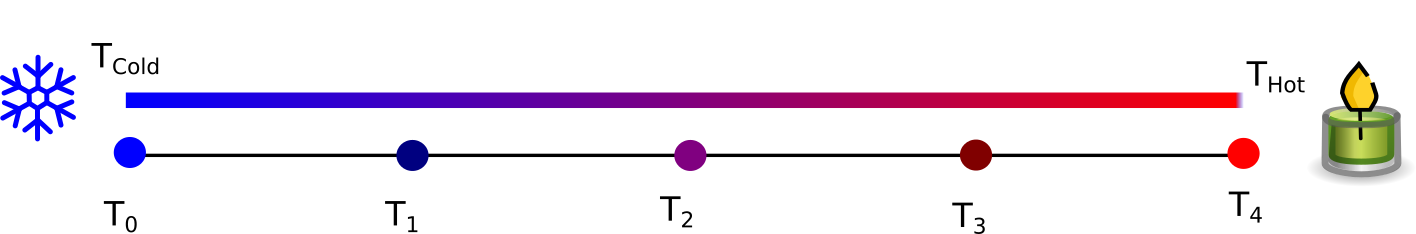
\includegraphics[width=\textwidth]{./images/mesh/general_mesh_diagram.png}
\caption{An example of a continuous problem broken up (or meshed) into a series of discrete points.}
\label{fig:emeshdiagram}
\end{figure}

\section{Different meshes for different problems}

In simple terms OghmaNano solves three physical models, the optical model describing light, the thermal model describing thermal effects and the electrical model describing electrical effects. The physical effects from each of these three models often happen on different length scales so need different meshes. For example:

\begin{itemize}
  \item Electrically interesting effects may only happen in the active layer of a solar cell (100 nm thick), so it is only worth solving the drift diffusion equations in this layer, however light interacts with all layers in the cell (1 $\mu$m thick) so the optical problem should be solved over the entire device. This means light should be modelled covering the whole device but electrical effects only in the active layer.
  \item A Quantum Well laser diode used for cutting steel may generate a lot of heat in it's Quantum Well (30 nm thick) and waveguide layers (1 $\mu$m) thick but heat will escape from device through a heat sink which may be a 1 cm thick block of copper. This means electrical effects should be modelled within the device on (1 $\mu$m) scale the but thermal effects should be modelled on the cm scale.
\end{itemize}

Thus different effects need to be simulated on different length scales. Furthermore, you electrical device structure may have some very thin layers such as contact layers or interface layers which are only a few nanometres thick. Optically these layers are far below the wavelength of light so you don't need to worry about them from the optical perspective, but electrically they are very important as they define the current voltage characteristics of the device. Thus you would want to use a very fine electrical mesh over the layer to make sure they were modelled accurately from the electrical stand point but you could use a very wide optical mesh that skips the layers. 

In general OghamNano interpolates between the three meshes, so for example if you set up an thermal profile using a temperature mesh, and the temperature values are needed in the electrical problem the values are transferred through interpolation. You don't need to worry about this as a user. The same is true for the optical simulation values of Generation rate etc. are interpolated between from the optical mesh to the electrical mesh as needed.

\section{The three meshes of OghmaNano}
The thermal, optical and electrical ribbons are shown below in Figure \ref{tab:mesh_ribbons},  it can be seen that in each of these ribbons is a a mesh button, where the thermal, optical and electrical meshes can be defined.

\begin{figure}[H]
\centering
\begin{tabular}{ c }
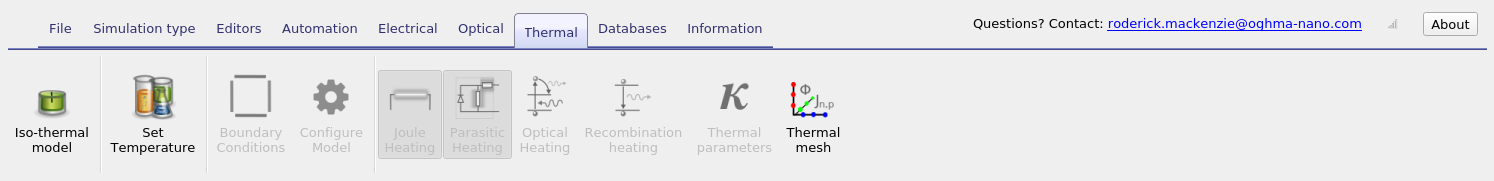
\includegraphics[width=0.9\textwidth,height=0.1\textwidth]{./images/mesh/mesh_0.png}  \\
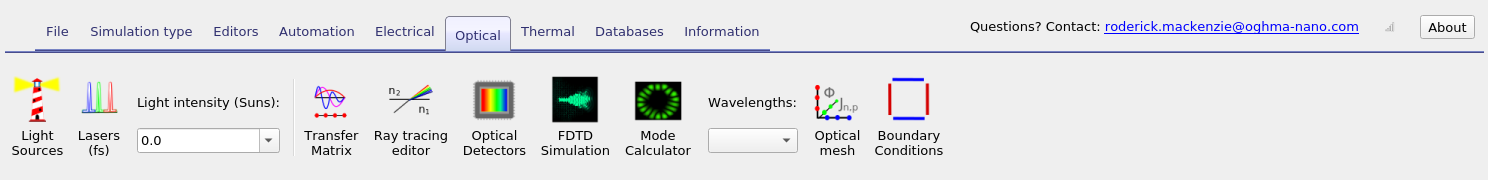
\includegraphics[width=0.9\textwidth,height=0.1\textwidth]{./images/mesh/mesh_1.png}  \\
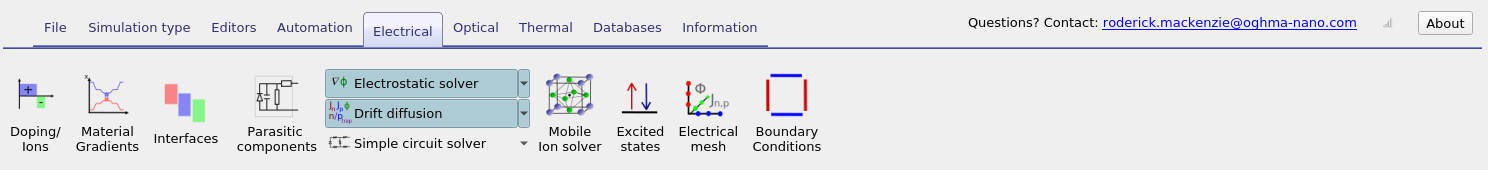
\includegraphics[width=0.9\textwidth,height=0.1\textwidth]{./images/mesh/mesh_2.png}  \\
\end{tabular}
\caption{The thermal, electrical and optical ribbons.}
\label{tab:mesh_ribbons}
\end{figure}


\subsection{Electrical mesh}
If you click on the electrical mesh button in the electrical ribbon of the main window a window looking like Figure \ref{fig:emesh} will appear. The buttons marked 1D, 2D and 3D at the top of the window in Figure \ref{fig:emesh} can be used to toggle the simulation between 1D, 2D and 3D modes.  In this example the mesh is set up for a 2D OFET simulation, so \emph{y} and \emph{x} are depressed. Note, if you want to do 2D or 3D simulations you are best off using a default 2D simulation, such as the OFET simulation.  This is because to do 2D/3D simulations, a special newton solver configuration will be needed. The tables that looks like a spreadsheet is used to configure the mesh. The columns \emph{thickness} and \emph{mesh points}, determine the thickness of the mesh layer and the number of points on the mesh layer. The column, \emph{step multiply} by how much to grow each step.  For the second row of the x mesh the step multiplier is set to 1.1 which means the distance between the points will grow by 10\% each mesh point. The buttons marked left/right, defines on which side the mesh layer is generated from.  The resulting meshes are plotted in the graphs at the bottom of the window.

\begin{figure}[H]
\centering
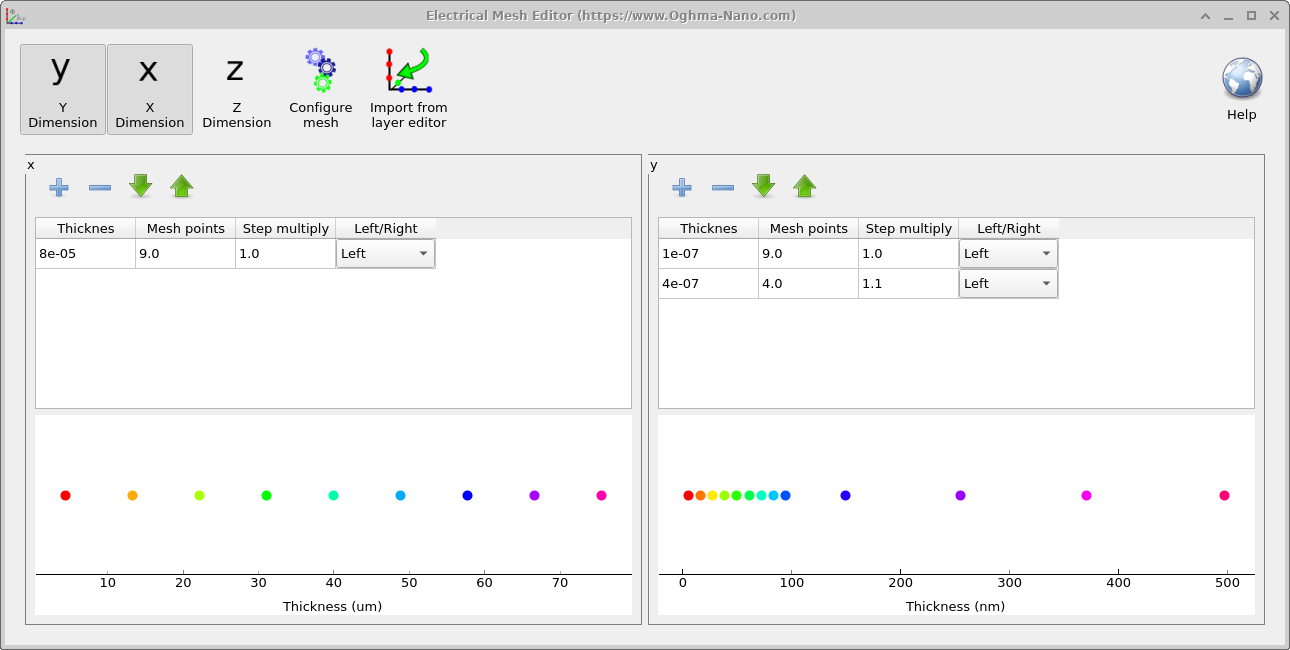
\includegraphics[width=0.8\textwidth]{./images/mesh/electrical_mesh_window.png}
\caption{The electrical mesh editor showing the mesh for a 2D OFET simulation.}
\label{fig:emesh}
\end{figure}

The button called \emph{Import from layer editor} clears the y-electrical mesh and imports all the layers from the layer editor giving them four mesh points each. This is useful when setting up complex structures with many layers such as laser diodes.
 
\subsection{Optical mesh}
The optical mesh window is shown below in Figure \ref{fig:optical_mesh}, this is more or less identical to the electrical mesh window except it also has a panel to configure which wavelengths are simulated in a simulation. These wavelengths are used in ray tracing, FTDT simulations and transfer matrix simulations. In any simulation where a wavelength range is defined this mesh will be used.

\begin{figure}[H]
\centering
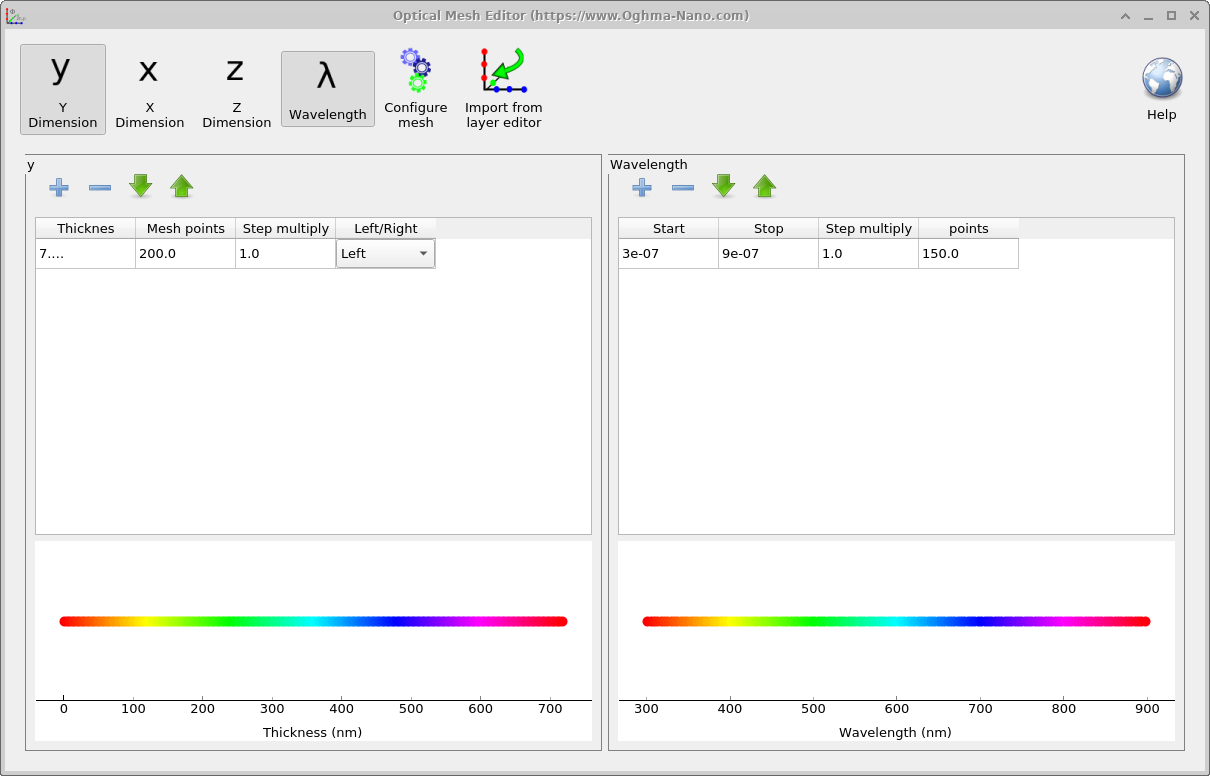
\includegraphics[width=0.8\textwidth]{./images/mesh/optical_mesh_window.png}
\caption{The optical mesh editor showing the number of points in position space and the number of wavelength points used for the optical simulations.}
\label{fig:optical_mesh}
\end{figure}

\subsection{Thermal mesh}
This will generally be handled automaticity for you. And you will only need to consider the thermal mesh when you turn on self heating in the device. Some parameters such as 
 
\section{The electrical mesh in detail}
A picture of the electrical mesh is given below \ref{fig:electrical_mesh_diagram} note the mesh does not start at zero but half a mesh point into the device.

\begin{figure}[H]
\centering
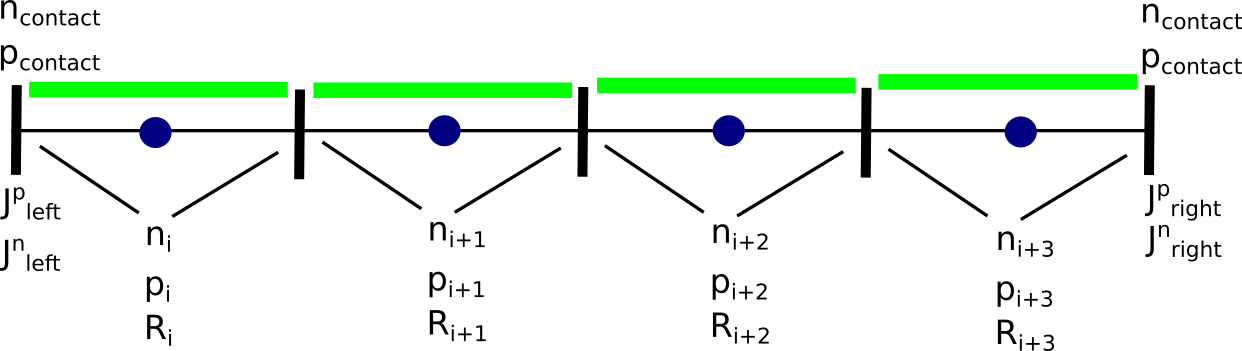
\includegraphics[width=0.8\textwidth]{./images/mesh/electrical_mesh_diagram.png}
\caption{A 1D diagram of the mesh}
\label{fig:electrical_mesh_diagram}
\end{figure}

\pagebreak
\section{When do I need to worry about meshing in OghamNano?}
\subsection{Electrical mesh}
You will already know that the layer editor is used to split the device up into layers of different materials (See section \ref{sec:layereditor}).  Some of these layers will have the layer type \emph{active}.  An \emph{active} layer is a layer over which the electrical model will be applied.  The electrical model needs a finite difference mesh to to be setup over the active layer for it to work. The length of the mesh and the length of the active layer must be exactly the same or you will get an error.  OghmaNano will try to do this for you in most cases, so generally speaking for simple problems you will not have to think about meshing. However if one starts adding multiple active layers you may have to define your own mesh. Other times when you will need to worry about meshing is when you are interested in cutting down the number of mesh points used to speed your simulation up or when you want to make your simulation more accurate by increasing the number of mesh points.

\subsection{Optical mesh}
You will need to play with the optical mesh if you want to change the wavelength range over which light is simulated in the device. You will also want to change the number of points in position space in this mesh if you want more accurate (more mesh points) or faster (more mesh points) optical simulations.

\subsection{Thermal mesh}
If you want to do simulations with trap states with self heating turned on you will need to define a thermal mesh, otherwise this will be taken care of for you.

\pagebreak
\section{Meshing tips}
\subsection{Should I be simulating in 1D, 2D or 3D?}
When deciding if you should perform 1D, 2D or 3D, simulations, consider the dimensionality of your problem.  For example if you consider a solar cell, it is only a few micros thick, and there is rapid variation in the structure, charge densities, mobilities, and doping as a function of depth (y).  However, the structure will not vary very in the lateral (xz) plane.  Therefore, in general  to capture all interesting effects present within a solar cell one only needs a 1D model.  If one now considers OFETs, there is both vertical an lateral current flow, therefore one can not get away with a 1D model any more, as one must simulate both vertical current flow, and current between the source and the drain, thus one needs a 2D simulation.  As the number of dimensions increases, computation speed will decrease, therefore my general advice is to use the minimum number of dimensions possible to solve your problem.

In short try to make your simulation as simple as possible as it will save you time and effort.  Generally the following geometries could be used for various types of devices:

\begin{table}[H]
\begin{center}
\begin{tabular}{ |c|c|c| } 
 \hline
	Device type			& 	Number of dimentions  \\ 
 \hline
	$Solar cells$ 		&	1D \\ 
	$Optical filter$	&	1D\\ 
	$OFET$ 				&	2D\\ 
 \hline
\end{tabular}
\caption{How many dimensions should I use to simulate my device.}
\end{center}
\end{table}

\subsection{Speed v.s. accuracy}
When setting up your device in OghmaNano you should try to:
\begin{itemize}
  \item Minimize the number of mesh points to improve computation speed but not go so low that accuracy is sacrificed.
  \item Realise that more mesh points does not necessarily mean a more accurate simulation. Especially in the electrical model the equations are discretized as not to lineally interpolate between mesh points, instead the actual differential equations are solved as boundary value problems between the mesh points. This means you can sometimes get away with surprisingly few mesh points (very fast simulations) and still get quite nice results.
  \item Don't be afraid to really reduce the number of mesh points when testing out fitting or trying to understand device performance.  This will give you a very fast simulation. You can always go back later and add more mesh points.
\end{itemize}

